% !TEX root = ../../report.tex

\section{Recommendation Methods}
\label{sec:rec-models}

The section will introduce the different recommendation methods included in our
experiments. We have included some simple non-personalized methods in addition
to the one-class collaborative filtering methods which will be used as baselines in
our experiment. Since we want to compare traditional methods with the one-class
collaborative methods we have chosen state-of-the-art solutions from both classes
to minimize the differences.


% Since our requires us to test multiple recommender systems to get a
%better overview of added value of including implicit factors and finally our implicit ratings.
% We have also chosen to
%include some simpler non-personalized methods to be used as baseline models to
%assess whether the current system is ready for a personalized recommendation
%system. Similarly to assess the improvement, if any, over the simple
%non-personalized methods for cold-start recommendations.  E.g. one could
%imagine to final system to leverage multiple recommendation techniques. When
%users are new to the system they are recommended the most popular items, until
%enough data is collected to start providing personalized recommendations.  This
%system could be complemented by pre-computed item similarities for
%recommendations in the context of the user \emph{examining} an item. If the
%cold-start performance of these simpler models outperform the more
%sophisticated ones included in our experiments, why not just use them? However,
%our greatest problem was to find methods which in some ways could bridge the
%broken divide between binary and non-binary recommendation systems to make our
%results valid. Our solution to this is to include those methods that are
%considered state-of-the-art from both classes in an attempt to bridge this
%highly \emph{unfortunate} weakness in our experiment.


\subsection{Extracting Content-Features}

To extract features for content-based recommendations we closely examined the content in the product database.
The product descriptions had five fields in particular that we found interesting: price, brand, title, description
and meta-description. The first two only contain one value and the three latter are made up of text.
Finding inspiration from the work on Ghani et. al. \cite{ghani2002building} and more closely studying the top keywords
found in the product description we decided to extract the following features:

\begin{itemize}
\item Price: grouped into price brackets
\item Brand or storename
\item Category: e.g. dress, jacket, top, pants and boots
\item Material: e.g. cotton, wool, polyester, leather
\item Style: e.g. classic, modern, comfy, sexy
\item Color
\end{itemize}

To extract the product-type, material, style and color we analyzed the content of the title, description and meta-description
fields extracting the most used keywords after removing the stopwords, which we combined and grouped for the different
attributes. Since descriptions and titles could be either in Norwegian or in English we had to include the words from
both languages. We also experimented with stemming from the nltk software package in python, but since it did not
improve our results it was not used in the final implementation. E.g. to determine if a product-type falls under
the \emph{sweater} category we check for the following keywords: \emph{sweater, cardigan, jumper, hoody , genser and genseren}.
The price and the brand of an item is stored in its own field, making it an easy task to extract. \newline

It was a pleasant surprise to find out that 5,060 out of 5,855 or 86.4\% of the items could be found in the
product database and be assigned features. The following our feature extraction results:

\begin{table}[H]
	\centering
	\begin{tabular}{l l}
	\toprule
	Attribute & Percentage  \\ \midrule
	Price 			& 1.000 \\
	Brand 			& 0.742 \\
	Category 		& 0.628 \\
	Material 		& 0.408 \\
	Style 			& 0.314 \\
	Color 			& 0.162 \\
	\bottomrule
	\end{tabular}
    \caption[Extracted content features]{Exteacted content features in dataset}
	\label{table:extracted-content-features}
\end{table}

Price, brand and product-type can be found for \emph{most} items, while material style
and color could only be found for a minority of the items. The dataset is in no way ideal
for content-based recommendation as it highlights on of the main weakness of content-based
methods, namely that they require rich descriptions of items to build well informed user
profiles. As mentioned in \cite{meyer2012recommender} this is most often not the case in
real applications. The content-features will be used to to test our one content-boosted collaborative
filtering method \cite{Gantner2010} in addition to being used by our filterbots to generate ratings based
on content-features.

\subsection{One-Class Recommenders}

This subsection will describe the algorithms used on the binary datasets. One-class Collaborative
filtering methods uses only binary data of the user's interaction to generate recommendations.
In addition to the methods described a user-based collaborative filtering model will be used.

\subsubsection{Most-popular Recommender}

We developed a simple most-popular recommender that uses result dithering to \emph{randomize}
the recommendations to the users. Dithering adds \emph{noise} to the algorithm, which permutes
the results in such a way that the top few results have a high probability of remaining on the top spots,
but as one goes deeper into the results, the degree of mixing increases dramatically. It is important to
note that dithering is \emph{guaranteed} to make off-line performance worse, but is likely to make the
actual performance better as the user is not presented with the same list of recommendations every
time. We experimented with two different methods of dithering:

\begin{itemize}
\item $Score = log_2(rank+x) - runif(y, z)$
\item $Score = log_2(rank+x) - y*rexp(z)$
\end{itemize}

The $runif$ function draw samples from a uniform distribution where $y$ specifies the lower boundary
of the output interval and $z$ specifies the upper boundary. The probability density function of the
uniform distribution is $P(x) = \frac{1}{z-y}$ anywhere within the interval $[y, z]$, and zero elsewhere.
The $rexp$ function draws a random number from an exponential distribution, where $z$ specifies the
$\lambda$ value, which is set to $\frac{1}{z}$. The following figure shows the exponential probability
density function given different $\lambda$ values:

% Vertical alignment of equation and plot.
\begin{figure}[H]
\label{fig:expdist}
  \centering
  \noindent\begin{minipage}{.45\textwidth}
    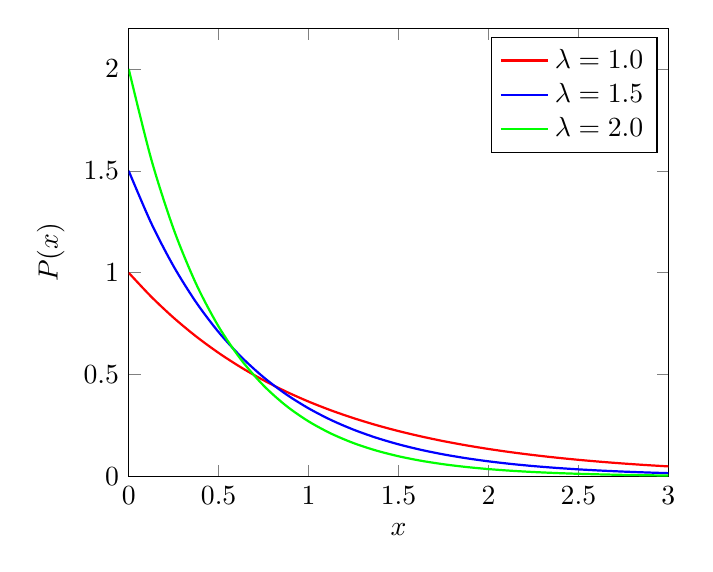
\begin{tikzpicture}
      \begin{axis}[
      	xlabel={$x$},
      	ylabel={$P(x)$},
      	ymin = 0, ymax=2.2, xmin=0, xmax=3,
      	legend entries={$\lambda=1.0$,$\lambda=1.5$,$\lambda=2.0$},
      	domain=0:3,
      ]
      \addplot[thick,smooth,red]{exp(-x)};
      \addplot[thick,smooth,blue]{1.5*exp(-1.5*x)};
      \addplot[thick,smooth,green]{2.0*exp(-2.0*x)};
      \end{axis}
    \end{tikzpicture}
    \end{minipage}
    \begin{minipage}{.45\textwidth}
      \begin{align}
        \label{exponential propability density function}
        rexp = \lambda e^{-\lambda x}
      \end{align}
      \end{minipage}
    \caption{Exponential probability density function}
\end{figure}


Given $x=5$, $y=0$ and $z=6$ using the uniform distribution dithering function we get the following
permutations in 10 runs:


\begin{table}[H]
	\centering
	\begin{tabular}{*{11}l}
	\toprule
	\multicolumn{1}{l}{\#Run} & \multicolumn{10}{l}{Result} \\ \midrule
	1 	& 8 & 3 &  24 &  20 &  1 &  19 &  22 &  15 &  42 &  36 \\
	2 	& 2 &  0 &  1 &  32 &  20 &  3 &  35 &  34 &  43 &  10 \\
	3	& 7 &  1 &  3 &  12 &  2 &  25 &  0 &  9 &  24 &  27\\
	4	& 0 &  4 &  3 &  5 &  7 &  16 &  26 &  22 &  13 &  33\\
	5	& 0 &  10 &  8 &  1 &  15 &  5 &  30 &  17 &  11 &  35\\
	6	& 7 &  4 &  6 &  12 &  2 &  1 &  19 &  0 &  27 &  9\\
	7	& 1 &  5 &  0 &  2 &  9 &  3 &  20 &  12 &  4 &  31\\
	8	& 0 &  1 &  2 &  5 &  39 &  4 &  15 &  41 &  10 &  22\\
	9	& 4 &  6 &  0 &  3 &  1 &  29 &  36 &  31 &  35 &  20\\
	10	& 5 &  1 &  0 &  8 &  3 &  18 &  25 & 24 & 2 & 28\\
	\bottomrule
\end{tabular}
\caption{Most Popular Result Dithering - Uniform Distribution}
\end{table}

The numbers specify the items original position before the ditering, e.g. item 0 was originally
the highest ranked item, item 8 was originally ranked as number 9 and so on. Given $x=1$, $y=3.0$
and $z=2.5$ using the exponential distribution we get the following permutations of the original
ranking in 10 runs:

\begin{table}[H]
	\centering
	\begin{tabular}{*{11}l}
	\toprule
	\multicolumn{1}{l}{\#Run} & \multicolumn{10}{l}{Result} \\ \midrule
	1	& 2 &  4 &  0 &  35 &  3 &  1 &  15 &  72 &  9 &  5\\
	2	& 0 &  10 &  11 &  17 &  1 &  3 &  8 &  41 &  15 &  5\\
	3	& 44 &  1 &  0 &  15 &  9 &  4 &  5 &  59 &  26 &  2\\
	4	& 0 &  98 &  1 &  4 &  2 &  41 &  8 &  26 &  11 &  94\\
	5	& 0 &  6 &  1 &  2 &  70 &  4 &  19 &  14 &  8 &  3\\
	6	& 2 &  5 &  0 &  16 &  15 &  18 &  1 &  3 &  32 &  6\\
	7	& 2 &  65 &  4 &  0 &  3 &  45 &  8 &  1 &  48 &  36\\
	8	& 3 &  49 &  5 &  0 &  2 &  82 &  8 &  77 &  11 &  4\\
	9	& 0 &  1 &  21 &  8 &  4 &  85 &  2 &  6 &  47 &  3\\
	10	& 0 &  1 &  21 &  70 &  11 &  20 &  2 & 10 & 9& 3 \\
	\bottomrule
\end{tabular}
\caption{Most-Popular Result Dithering - Exponential Distribution}
\end{table}

As you can see the lists generated are quite different. The uniform distribution has a lower occurence of higher
numbers in the lists, but it also has a smaller occurrence of smaller numbers. The exponential distribution
goes as far as including an item that originally was ranked 98th. This is due to the fact that the exponential
distribution can output large values, in theory up to infinity, with a decreasing probability.
However, you can also see that the highest ranked items is consistently found at the top of the list
for the exponential function.
To get a clearer image of their differences consider the following figure which shows the minimum, maximum and average position of
the first 10 items for 100 over recommendations using the same parameters as above:

\pgfplotstableread{
x    y    	y-max  	y-min
0 	1.40 	3.60 	1.40
1 	3.18 	6.82 	3.18
2 	5.25 	6.75 	5.25
3 	6.40 	7.60 	6.40
4 	9.28 	10.72 	9.28
5 	10.77 	13.23 	10.77
6 	11.57 	12.43 	11.57
7 	13.73 	15.27 	13.73
8 	15.42 	13.58 	15.42
9 	16.04 	13.96 	16.04
}{\expdist}

\pgfplotstableread{
x    y    	y-max  	y-min
0	3.56	15.44	3.56
1	5.91	25.09	5.91
2	8.69	22.31	8.69
3	12.31	34.69	12.31
4	12.69	40.31	12.69
5	15.74	36.26	15.74
6	19.99	42.01	19.99
7	21.05	41.95	20.05
8	24.73	42.27	23.73
9	23.71	45.29	23.71
}{\uniformdist}

\begin{figure}[H]
	\label{fig:minmaxuniform}
	\centering
	\begin{tikzpicture}
	\begin{axis} [
		ymin=-5,
		xlabel={Original Position},
		ylabel={Position After Dithering},
	    symbolic x coords={0,1,2,3,4,5,6,7,8,9},
	    xtick=data
	]
	\addplot [only marks, red]
	  plot [error bars/.cd, y dir=both, y explicit, error bar style={line width=2pt}]
	  table [y error plus=y-max, y error minus=y-min] {\uniformdist};
	\addplot [only marks, blue]
	  plot [error bars/.cd, y dir=both, y explicit]
	  table [y error plus=y-max, y error minus=y-min] {\expdist};
	\end{axis}
	\end{tikzpicture}
	\caption[Average position of recommendations with dithering]{Minimum, maximum and average position of 10 first items over 100 recommendations for the exponential distribution dithering (blue) and uniform distribution dithering (red)}

\end{figure}

The figure show that the exponential distribution varies the position of the first items much less
than the uniform distribution, never putting the highest ranked item lower than number five in the
list while the uniform distribution puts it as far back as 20th. The values of $x$, $y$ and $z$ can be modified to
achieve the desired degree of mixing.

\subsubsection{One-Class Item-based Collaborative Filtering}

There are a number of different ways to compute the similarities between items given binary preference data.
Here we present one such method called \emph{log likelihood}, which is implemented in Mahout \cite{mahout}
Log Likelihood Similarity is used to score and analyze counts of events, particularly counts of when events occur together.
The counts you have in these situations are the following:

\begin{itemize}
\item $c_{11}$ the number of times two events have occurred together
\item $c_{12}$ and $c_{21}$ the number of times one occurred without the other.
\item $c_{22}$ the number of times something was observed that was neither.
\end{itemize}

Once you have these counts the log likelihood $G^2$ can be computed as follows:\newline

\begin{subequations}
$G^2$ = 2(matrixEntropy(c)-rowEntropy(c)-columnEntropy(c))
\begin{align}
	rowEntropy(c) = H(c_{11}, c_{12}) + H(c_{21}, c_{22}), \\
	colEntropy(c) = H(c_{11}, c_{21}) + H(c_{12}, c_{22}), \\
	matrixEntropy(c) = H(c_{11}, c_{12}, c_{21}, c{22}),
\end{align}
\end{subequations}

where $H$ is Shannon's entropy, which can be computed using the following formula:

\begin{equation}
H(X) = - \sum_{i} x_i log \frac{x_i}{N} = -N \sum_i \frac{x_i}{N} log \frac{x_i}{N}
\end{equation}

where $N$ equals $\sum_i x_i$. Using the above notation Shannon's entropy for $H(c_{11}, c_{21})$ gives us:

\begin{equation}
H = (c_{11} + c_{12})log(c_{11} + c_{12})-c_{11} log(c_{11}) - c_{12} log(c_{12})
\end{equation}

In addition to log likelihood we will also experiment with the cosine similarity model
found in MyMediaLite \cite{Gantner2011MyMediaLite}.

\subsubsection{BPR: Bayesian Personalized Ranking}

BPR presented by Rendle et. al. \cite{Rendle2009} can be used to learn the latent factors of a
latent factor model using binary implicit feedback. For our experiment we have used to implementation
found in MyMediaLite \cite{Gantner2011MyMediaLite}. Bayesian Personalized Ranking was designed for the item
prediction task and optimized for ranking using implicit feedback such as e.g. purchases in an online shop.
The task of the recommender system is to provide the user with a personalized ranking $>_c \subset I^2$ of all
items, where $>_c$ has to meet the properties of a total order. Finding the personalized ranking for all items
$s \epsilon S$ is to maximize the following posterior probability where $\theta$ represents the parameter vector
of an arbitrary model in our case a matrix factorization model.

\begin{equation}
p(\theta | >_c) \propto p(>_c | \theta) p(\theta)
\end{equation}

Where $>_c$ is the desired but latent preference structure for user $c$. All users are presumed to act
independently of each other. The ordering of each pair of items is assumed to independent of every other pair.
The generic optimization criterion for personalized ranking is as follows:

\begin{equation}
BPR(D_S) = \underset{\theta}{\arg\max} \sum_{(c,i,j)\epsilon D_s} ln \sigma(\hat{u}_{c,i}(\theta)-\hat{u}_{c,j}(\theta)) - \lambda \left\|\theta \right\|
\end{equation}

Here $D_s$ is the binary dataset used, $\sigma(x)$ is the logistic sigmoid function, $\theta$ represents
the model parameters, $\hat{u}_{c,s}$ is the predicted score for user $c$ and item $s$ and
$\lambda \left\|\theta \right\|$ is the regularization term. It reduces the model learning task to
a pairwise classification problem.\newline

BPR learns the model parameters $\theta$ as follows using stochastic gradient descent:

\begin{itemize}
\item Step 1: Draw (c,i,j) from $D_S$
\item Step 2: $\theta \leftarrow \theta + \alpha \left\lgroup \frac{\exp^{-\hat{x}_{cij}}}{1+\exp{\hat{x}_{cij}}}  \frac{d}{d \theta} \hat{x}_{cij} + \lambda_{\theta} \theta \right\rgroup$
\item Step 3: Repeat step 1 and 2 until convergence
\end{itemize}

where $\alpha$ is the learning rate and $\lambda_{\theta}$ is the regularization constant. BPR will hereby be
referred to as BPR-MF.

\subsection{Non-Binary Recommenders}

The following recommenders will be used to test our implicit ratings. In addition to the methods described,
traditional user-based and item-based collaborative filtering described in Section~\ref{subsubsec:memory-based} will
also be used.

\subsubsection{ALS-WR}

%Implicit Feedback Recommendation via Implicit-to-Explicit Ordinal Logistic Regression Mapping

ALS-WR is the only method which we have found that \emph{supports} implicit ratings, making
it a natural part of our experiment. For our experiment we have used the Mahout \cite{mahout} implementation.

Alternating-least-squares with weighted-$\lambda$-regularization (ALS-WR) was designed fro the Netflix Prize
Competition \cite{Netflix}, where it obtained an RMSE score of 0.8975, which was one of the best results based
on a pure method. As you may know, the Netflix Prize Competition was won using an ensemble of multiple predictors.

Alternating-least-squares is a method to solve Equation~\ref{equation:minimize}. Since both $q_{s}$ and $p_{c}$
are unknown, the equation is not convex. However if we fix one of the unknowns, the optimization problem becomes
quadratic and can be solved optimally. The ALS technique rotate between fixing the $q_{s}$'s and fixing the $p_{c}$'s.
When all the $p_{c}$'s are fixed, the system recomputes the $q_{s}$'s by solving a least-squares problem, and vica versa.
This ensures that each step decreases the error until convergence. What makes ALS favorable over the simpler and faster
stochastic gradient descent is two things. ALS can be parallelized since the system computes the $q_{s}$'s independently
of the other item factors, the same can also be applied to the user factors. The second case if for systems centered around
implicit data. Because the training set cannot be considered sparse, looping over each single training case as gradient descent
would not be practical, but ALS can efficiently handle such cases \cite{Hu2008}.\newline

ALS solves the low-rank matrix factorization as follows:

\begin{itemize}
\item Step 1: Initialize the matrix M by assigning the average rating for that movie as the first row, and a small random numbers for the remaining entries;
\item Step 2: Fix P, solve Q by minimizing the objective function (the sum of squared errors);
\item Step 3: Fix Q, solve by minimizing the objective function similarly;
\item Step 4: Repeat Steps 2 and 3 until a stopping criterion is satisfied.
\end{itemize}

Without regularization ALS might lead to overfitting due to the many free parameters. Regularization was
therefore introduced in the form of weighted-$\lambda$-regularization to prevent the model from overfitting.

\begin{equation}
f(P, Q) = \sum_{(c,s)\epsilon C} (u(c,s) - p^{T}_{c}q_{s})^{2} + \lambda (\sum_{c} n_{p_{c}} \Vert p_{c} \Vert ^{2} + \sum_{s} n_{q_{s}} \Vert q_{s} \Vert ^{2})
\label{WeightedLamba}
\end{equation}

where $n_{p_{c}}$ and $n_{q_{s}}$ denote the number of ratings of user $c$ and item $s$ respectively. $S_{c}$ denote
the set of items $s$ that user $c$ rated, then $n_{p_{c}}$ is the cardinality of $S_{c}$; similarly $C_{s}$ denotes
the set of users who rated item $s$, and $n_{q_{s}}$ is the cardinality of $I_{s}$. A given column of P, $p_{c}$ is
found by solving a regularized linear least squares problem involving the known ratings of user $c$, and the
feature vectors $q_{s}$ of the items that user $c$ has rated. Similarly, we can compute individual $q_{s}$'s via
a regularized linear least squares solution, using the feature vectors of users who rated item $j$, and their ratings of it.
The implicit feedback extension of the method is described in~\ref{implicit-als-wr}.

\subsubsection{Item-Average}

Item average is a simple recommender that always estimates the preference for an item to be the average of
all known preference values for that item. No information about the individual users is taken into account.
This recommender can therefore be considered a \emph{highest rated} recommender, as it is likely to recommend
the highest rated items. The following equation shows the rating prediction procedure:

\begin{equation}
\label{equation:itemaverageratingprediction}
u(c,s) = k * \sum_{c' \epsilon C} u(c',s)
\end{equation}

where $k$ is a normalization factor ($1/|C|$). This is very similar to collaborative filtering, except for
the fact that the user similarity $sim(c, c')$ has been taken out of the equation. This is the same as saying
that all user similarities are the same. It is also worth mentioning that this method is not suited for binary
ratings, is it need ratings to average on.

\subsection{Cold-start Solution}

Due to limitations, mainly in the form of a lack of additional data sources the cold-start solutions
we are currently able to experiment with is fairly limited. As we never got access to
user-data, we have to cross out RBLF and other methods requiring user features. This leaves us with
Naive Filterbots \cite{Park2006} which easily could be combined with our implicit ratings.

\subsubsection{Filterbots}
\label{implementation-filterbots}

The main reasons for experimenting with filterbots is simplicity, the fact that it easily could
be combined with our implicit ratings in addition to the fact that previous experiments \cite{Agarwal2009, Agarwal2010}
show that its performance is close to the state-of-the-art methods. It is worth to keep in mind that filterbots was
developed for traditional neighborhood collaborative filtering methods, and will therefore only be applicable given
that a neighborhood model is chosen as the core recommender. Filterbots can potentially help solve the cold-start user
problem by making it possible for new users to connect to pseudo users that capture the general underlying trends of the entire
user group. Filterbots were designed to improve performance when data is scare without degrading performance when the data
is plentiful.

Similarly as in \cite{Park2006} we decided to experiment with \emph{naive} global bots. The bots are \emph{naive}
in the sense that they are \emph{dumb} in the way they rate items, e.g. by only considering one item-attribute of the items.

We have currently implemented the following bots:

\begin{itemize}
\item BrandBot: rates all items based on the average brand rating
\item BrandBots: multiple bots that give all items of a specific brand a maximum rating
\item PopularityBot: rates all items based on their popularity
\item AverageBot: rates all items based on their average rating
\item CriticBot: $n$ critics among the most active users are selected and rate items based on the average
	  rating given by these critics.
\end{itemize}

The \emph{PopularityBot} estimates each rating using the following formula: $r(c,s) = log_{3}C_{s}$, where $C_{s}$ is the number of users which have rated the item and $3$ is a normalization constant that caps the ratings a little below 5, which is our maximum rating.
Compared to the work presented by Park et. al. we felt that the lack of high quality features was a limiting factor when designing the filterbots, as most features would not let us rate most ratings, and there is only so much information in the rating matrix.

The intuition behind the \emph{SingleBrandBots} is as follows, given that a user-based collaborative filtering algorithm is used:
when a new user \emph{rates} an item of a single brand it will be connected with one such bot. The user can then be recommended
items from this bot's list, meaning that the user can be recommended items of the same brand. Which in theory, should be better
than recommending some item from a random brand. Similarly, the \emph{PopularityBot}
will have rated the popular items highly meaning that new users that connect to this psuedo user will be recommended the
most popular items. For item-based methods it works a little differently as it only has an effect on the item-similarity matrix.
Since more item similarities can be defined due to the psuedo users, more neighbors for the target item can be chosen from the candidate set.

Both the \emph{AverageBot} and \emph{BrandBot} can be seen to incorporate the implicit rating factors such as recency into
the ratings generated. However, for the \emph{PopularityBot} and \emph{Critic} but we wish to implement additional functionality to ensure
that the new users are connected with items that are relevant right now and not consider outdated items or users which
are no longer active. Since we have access to timestamps we could e.g. make the \emph{PopularityBot} rate items based on
their popularity the last couple of weeks instead of over the entire dataset period. Similarly, critics can be selected
based on their activity the couple of weeks/months.

\subsection{Test Suite}

As many of our selected evaluation metrics not is implemented in the recommender system libraries used we implement our own test suite. It is a bash
script that takes the entire log file as input first transforming it to into a set of ratings, or blend of your choice before splitting it based on timestamps
or simply generating a random split. These outputs are then fed into either Mahout or/and MyMediaLite training the specified models and writing their predictions to file. Our evaluation suite then calculates all the metrics desired writing them out in a latex format. All in one command line call. Our evaluation suite currently supports nDCG, $MAP@K$, User and Item-Space Coverage, hLU, MPR, in addition to our own unique simple event evaluator. The current functionality is
highlighted in the listing below:

\begin{lstlisting}
$ ./testsuite.sh -h
Usage: ./testsuite.sh [options]

This program can do the following depending on the options provided:
  - Generate a set of implicit ratings based on an event log.
  - Recommend based on methods provided either by Mahout or MyMediaLite.
  - Evaluate the results yielding MAP@20, AUC and ROC.
  - Write the result to a latex-table, for easy exporting to a report.

OPTIONS:
  -a <filterbot settings> A string defining which filterbots to enable.
                          Defaults to '0,0,0,0,0'.
  -c                      Clean existing rating, prediction and scoring files
                          before running.
  -i <input file>         The absolute path to the event log file.
  -f <product features>   The absolute path to file containing all product
                          features obtained from the product DB.
  -d <product file>       Where to find product file with JSON-data, used with
                          cold-start splits. Defaults to 'generated/products.txt'
  -r <rank recommenders>  Which rank recommenders to user with MyMediaLite.
  -p <item recommenders>  Which item recommenders to use with MyMediaLite.
  -m <mahout algorithms>  Which recommender algorithms to use with mahout.
  -s <split type>         How to split test and training. Options: 'cold',
                          'time' or 'random'.
  -k <k values>           When using ItemKNN, control which k-values to use, as
                          a string of integers. E.g. '10 20 50'
  -b                      Convert all ratings to binary (all ratings to 1)
  -q                      Send stdout and stderr to /dev/null (except result)
  -t                      Split coldstart on time
  -l                      Run recommender on blend file only.
  -h                      Display this help-information.

RANK RECOMMENDERS:
  The following algorithms are available to use with the rank recommender
  provided by MyMediaLite:
    BiPolarSlopeOne, GlobalAverage, ItemAttributeKNN, ItemAverage, ItemKNN
    MatrixFactorization, SlopeOne, UserAttributeKNN, UserAverage
    UserItemBaseline, UserKNN, TimeAwareBaseline
    TimeAwareBaselineWithFrequencies, CoClustering, Random, Constant
    LatentFeatureLogLinearModel, BiasedMatrixFactorization, SVDPlusPlus
    SigmoidSVDPlusPlus, SocialMF, SigmoidItemAsymmetricFactorModel
    SigmoidUserAsymmetricFactorModel, SigmoidCombinedAsymmetricFactorModel
    NaiveBayes, ExternalRatingPredictor, GSVDPlusPlus

ITEM RECOMMENDERS:
  The following algorithms are available to use with the item recommender
  provided by MyMediaLite:
    BPRMF, ItemAttributeKNN, ItemKNN, MostPopular, Random
    UserAttributeKNN, UserKNN, WRMF, Zero, MultiCoreBPRMF
    SoftMarginRankingMF, WeightedBPRMF, BPRLinear, MostPopularByAttributes
    BPRSLIM, LeastSquareSLIM

MAHOUT RECOMMENDERS:
  The following methods are available when using Mahout:
    svd, itembased, userbased, itemuseraverage, loglikelihood, itemaverage

Examples:
  Split randomly and calculate the itemaverage with mahout:
  ./testsuite.sh -i ../somefile.tab -s random -m 'itemaverage'

  Split on time and use itemKNN with various K-values to do recommendations:
  ./testsuite.sh -i ../somefile.tab -s time -p 'ItemKNN' -k '10 20 50'

  Split with cold start and use some filterbots:
  ./testsuite.sh -i ../somefile.tab -s cold -m 'userbased' -a '1,1,1,0,0'
\end{lstlisting}
